% Sollte größter Teil werden
% - High level overview?
% - Wie läuft das auf meinem System?
% - Code Dokumentation / Entwicklerdokumentation

%%%%%%%%%%%%%%%%%%%%%%%%%%%%%%%%%%%%%%%%%%%%%%%%%%
% Abschnitt - Grober Überblick
%%%%%%%%%%%%%%%%%%%%%%%%%%%%%%%%%%%%%%%%%%%%%%%%%%

%%%%%%%%
% Low level
% was muss ich als entwickler wissen
% tiles, parallelisierung, structs/klassen, struktur des projekts

% Zuordnung klasse -> Dokumentation
% backend
%   *.main.cpp, init -> Niels DONE
%   include Ordner und CMake -> Niels DONE
%   balancer + tests -> Florian
%   mandelbrot -> Florian (außer MandelbrotSIMD -> Niels DONE)
%   actors
%      Worker -> Tobi
%      Host
%         websocket-funktionen -> Niels
%         Rest -> Tobi
%           + Parallelisierungskonzept (+ welche MPI Method, warum)
%   structs/Netzwerk -> Tobi/Niels/Florian
%   dev-environment (was ist docker und wie/warum) -> Max
% frontend
%    connection -> Niels
%    tileDisplay -> Max
%        TileDisplay.ts
%            Prinzip 
%            genauer Ablauf/Funktionen
%               + Shader
%        WorkerLayer.ts
%           + Gruppierung
%        MatrixView.ts + RegionOfInterest.ts
%        Project.ts
%    visualization -> Niels
%    misc -> Max

\section{Dokumentation der Implementierung}

\subsection{Implementierung des Backends}

Zur hardwarenahe Berechnung der Mandelbrotmenge wird ein sogenanntes Backend gestartet.
Das in C++ programmierte Teilprojekt nimmt Rechenaufträge von einem Nutzer durch ein Frontend entgegen (auch
ein solches wird bereitgestellt), zerlegt sie und verteilt sie per MPI auf dedizierte Rechenknoten.
Dazu besteht das Backend aus zwei ausführbaren Dateien, \verb|host| und \verb|worker|.

\subsubsection{Inkludierte Header und CMake Anweisungen}

Sämtliche Headerdateien sind ohne Untergruppierung im Ordner \verb|include| des Projektes abgelegt.

Sie werden zusammen mit den Header-Bibliotheken \verb|rapidjson| und \verb|websocketpp| sowie der vorkompilierten
Bibliothek \verb|boost_static| von CMake eingebunden um das Projekt zu builden.

Für einen erfolgreichen Build wird CMake einer Version von mindestens 3.7.0 und die C++11 Standards vorrausgesetzt.
Ergebnis des Builds sind die ausführbaren Dateien \verb|host| und \verb|worker| welche die
beschriebenen Funktionen innerhalb des Backends umsetzen.

Eine detailliertere Beschreibung ist im Anhang zu finden.

\subsubsection{Mainfunktion und Initialisierung}

Zur Initialisierung der Prozesse muss zunächst die MPI-Umgebung aktiviert und abgerufen werden.
Dies geschieht für beide Programme gleich, über die Initialisierungsfunktion in \autoref{src:init.cpp}.
Sie erwartet lediglich eine Beschreibung des Prozesses für den Log und eine Initialisierungsfunktion,
die erst zurückkehrt, wenn das Programm abgeschlossen ist und MPI beendet werden soll.
Die Funktion muss als Parameter den Rang bzw. die Id des aktuellen MPI-Prozesses und die Anzahl der initialisierten
Prozesse entgegen nehmen.

\subsection{Implementierung der Lastbalancierung}\label{sec:load_balancing}
Der Implementierung der Lastbalancierung liegen die in \autoref{sec:load_balancing_concepts} beschriebenen Konzepte zugrunde.
Wichtig bei der Umsetzung dieser ist, dass der garantierte Teiler (\verb|guaranteedDivisor|) von Höhe und Breite der Teilregionen dem der angeforderten Region entspricht (vgl. \autoref{fig:concept_coordinates}).
Eine Tile (ein Bereich mit Breite und Höhe gleich dem garantierte Teiler\footnote{Eine Region lässt sich also immer in eine ganzzahlige Anzahl von Tiles aufteilen, vgl. \autoref{fig:leafletTiles}}, die Bezeichnung \textit{Tile} kommt aus dem Frontend) muss also als atomare Einheit betrachtet werden, da es sonst im Frontend zu Schwierigkeiten bei der Darstellung kommt.

Die Klassenstruktur der Lastbalancierer entspricht dem Strategy-Pattern (vgl. \cite{gamma_design_1995} S. 315-323). So kann der Balancierer zur Laufzeit leicht gewechselt werden und auch die Erweiterung des Projekts um eine neue Strategie gestaltet sich einfach.
Was dabei genau beachtet werden muss findet sich im Teil Erweiterung (\ref{lastbalancierung_erweiterung}).

\subsubsection{Naive Strategie}

Die naive Strategie (\verb|NaiveBalancer| und \verb|RecursiveNaiveBalancer|) lässt sich in beiden Varianten recht einfach nach dem oben beschriebenen Konzept umsetzen.
Zusätzlich wurde noch \verb|ColumnBalancer| implementiert, dabei handelt es sich um eine Variante des nicht-rekursive Ansatzes, die nur Spalten erzeugt.
Die Erhaltung des garantierten Teilers wird dadurch erreicht, dass die Höhe und Breite der Teilregionen auf ein Vielfaches dieses Teilers gesetzt werden.
Diese können bei der nicht-rekursiven Variante vor der eigentlichen Aufteilung bestimmt werden.
Da sich $\frac{width}{guaranteedDivisor}$ nicht unbedingt durch die Anzahl an Workern teilen lässt, kann es sein, dass einige Teilregionen um \verb|guaranteedDivisor| Pixel breiter sind.
Selbiges gilt für die Höhe.

Bei der rekursiven Variante wird mithilfe folgender Kriterien entschieden, ob horizontal oder vertikal geteilt wird:

\begin{itemize}
	\item Region vertikal oder horizontal nicht mehr teilbar (d.h. \verb|width| bzw. \verb|height| $\leq$ \verb|guaranteedDivisor|): Teile in die andere Richtung.
	\item Region vertikal und horizontal unteilbar: Erzeuge eine leere Region für die zweite Hälfte.
	\item Sonst: Teile parallel zur kürzeren Seite. Dies gibt dem Lastbalancierer mehr Möglichkeiten die Trennlinie zwischen den Teilregionen zu setzen, was zu einer genaueren Teilung führt.
\end{itemize}

Die Teilung an sich funktioniert wie die nicht-rekursive Aufteilung auf zwei Worker.
Der Rekursionskontext (\verb|struct BalancingContext|) wurde extern definiert, da dieser für die Strategie mit Vorhersage wiederverwendet wird.

\subsubsection{Strategie mit Vorhersage}

Auch diese Strategie (\verb|PredictionBalancer| und \verb|RecursivePredictionBalancer|) folgt den oben beschriebenen Konzept.
Allerdings wurde die Berechnung der Vorhersage in eine eigene Klasse ausgelagert, da die Berechnung der Vorhersage für die rekursive und die nicht-rekursive Variante gleich ist.
Für die Berechnung der Vorhersage ist es notwendig, dass bei der Erststellung eine Referenz auf ein \verb|Fractal|-Objekt (siehe \ref{sec:mandelbrot_calculation}) übergeben wird.

\paragraph*{Bestimmung der Vorhersage}\label{par:predicter}
% predicter
Die Vorhersage (\verb|struct Prediction|) wird von der Klasse \verb|Predicter| angestellt.
Dazu wird die Region in einer sehr viel geringeren Auflösung berechnet.
Die benötigte Anzahl an Iterationen wird jeweils pro Tile abgespeichert.
So wird sichergestellt, dass der garantierte Teiler auch nach der Aufteilung noch gilt, da die Balancierer die Vorhersage Eintrag für Eintrag verarbeiten.
Die Genauigkeit der Vorhersage kann über das Attribut \verb|predictionAccuracy| gesteuert werden:
\begin{itemize}
	\item $predictionAccuracy > 0$: $(predictionAccuracy)^2$ Pixel werden pro Tile berechnet. Die Summe der Iterationen für die einzelnen Pixel ergibt die Vorhersage für die Tile.
	\item $predictionAccuracy < 0$: Für $(predictionAccuracy)^2$ Tiles wird ein Pixel in der Vorhersage berechnet. Es erhalten also mehrere Tiles diesselbe Vorhersage.
	\item $predictionAccuracy = 0$: Unzulässig, es wird ein Null-Pointer zurückgegeben.
\end{itemize}
Zusätzlich beinhaltet die Vorhersage die Summen der benötigten Iterationen pro Spalte und Zeile, sowie die Gesamtsumme.
So wird vermieden, dass diese während des Balancierens immer neu berechnet werden müssen.

\paragraph*{Nicht-rekursive Variante}\label{lastbalancierung_vorhersage}
% non-recursive prediction
Für die nicht-rekursive Aufteilung wird die Region erst in Spalten aufgeteilt und in einem zweiten Schritt wird dann die horizontale Unterteilung in Teilregionen vorgenommen.
Da die beiden Schritte analog zueinander sind wird hier nur das Aufteilen in Spalten anhand des Pseudocodes in \autoref{src:prediction_pseudo} beschrieben.

Die optimale Rechenlast pro Spalte (\verb|desiredN|) berechnet sich nach \autoref{equ:desiredN} wobei die Anzahl der Worker durch die Anzahl an Spalten ersetzt werden muss.
Als Abschätzung der Gesamtrechenlast wird die Gesamtsumme der Vorhersage verwendet.
Eine Spalte, die als leere Region beginnt, wird nun solange um eine Spalte von Tiles vergrößert bis die optimale Rechenlast erreicht oder überschritten wird.
Dazu müssen die Spaltensummen der Vorhersage aufaddiert werden.
Um Lücken auszuschließen werden die Grenzen der Spalten explizit aufeinander gesetzt, d.h. bei zwei benachbarten Teilregionen entspricht die obere Grenze der Einen der unteren Grenze der Anderen.
Damit es auch für die Aufteilung in Teilregionen eine Vorhersage gibt, wird eine Kopie der Vorhersage erstellt, welche nur die Werte für die aktuelle Spalte enthält (nicht im Pseudocode).

\begin{figure}[!h]
	\lstinputlisting[language=python, caption={Aufteilung in Spalten im Pseudocode}, label={src:prediction_pseudo}]	{./code/predictionbalancer.pseudo}
\end{figure}

Im eigentlichen Code wurden ein paar Optimierungen am Pseudocode vorgenommen.
Um float-Ungenauigkeiten beim wiederholten Addieren zu minimieren werden die Werte in \verb|cur| nicht aufaddiert, sondern aus den Zählern berechnet.
Außerdem werden die Spalten ohne Zwischenspeicherung in die nötigen Teilregionen aufgeteilt.
Zusätzlich wird \verb|desiredN| nach jeder abgeschlossenen Spalte für die Verbleibenden neu berechnet, da es sehr unwahrscheinlich ist, dass dieser Wert genau erreicht wird.

\paragraph*{Rekursive Variante}
% recursive prediction
Die rekursive Variante der Strategie mit Vorhersage verwendet dasselbe Rekursionsschema wie ihr naives Gegenstück.
Also wird auch die Entscheidung, ob horizontal oder vertikal geteilt werden soll, auf die gleiche Art und Weise gefällt.
Der Unterschied zwischen den beiden Strategien liegt also hauptsächlich in den beiden Methoden zur Aufteilung.

Bei dieser Strategie werden die Regionen nicht einfach halbiert, sondern in zwei Teile aufgeteilt, die laut der Vorhersage ähnlich rechenintensiv sind.
Dazu wird ähnlich vorgegangen, wie bei der \hyperref[lastbalancierung_vorhersage]{nicht-rekursiven Variante} für die Aufteilung auf zwei Worker.
Deshalb profitiert diese Strategie auch besonders davon, dass immer parallel zur kürzeren Seite geteilt wird, da die Vorhersage in diese Richtung feingliedriger ist.
Dies liegt daran, dass weniger Tiles der Vorhersage zu einer Spalte bzw. Zeile zusammengefasst werden müssen als wenn parallel zur längeren Seite aufgeteilt werden würde.
Allerdings wird hier, wenn möglich, sichergestellt, dass beide Teilregionen groß genug sind um jeweils auf die Hälfte der Worker aufgeteilt zu werden, da ansonsten unnötigerweise leere Regionen entstehen.
Es ist hierbei auch wichtig die Vorhersage so zu teilen, dass es für jede Hälfte eine Vorhersage gibt, die dann an den rekursiven Aufruf übergeben werden kann.

\subsubsection{Erweiterung}\label{lastbalancierung_erweiterung}

Da die Lastbalancierung nach dem Strategy-Pattern realisiert ist, gestaltet sich die Erweiterung um eine neue Balancierungsstrategie recht einfach.
Zuerst muss eine Unterklasse von \verb|Balancer| (\autoref{src:Balancer.h}) erstellt werden, um ein gemeinsames Interface zu ezwingen und somit die polymorphe Nutzung der neuen Klasse zu ermöglichen.

\begin{figure}[h!]
	\lstinputlisting[caption={Das gemeinsame Interface der Lastbalancierung}, label={src:Balancer.h}, firstline=7, lastline=11]{../../backend/include/Balancer.h}
\end{figure}

Danach wird die neue Strategie über die Methode \verb|BalancerPolicy::chooseBalancer| verfügbar gemacht.
Dazu muss sie mithilfe der statischen Variablen \verb|Klassenname::NAME| benannt werden.
\verb|BalancerPolicy| muss nun so erweitert werden, dass, bei Eingabe des vorher festgelegten Namens, ein neues Objekt der entsprechenden Klasse zurückgegeben wird.

\paragraph*{Bedingungen an Balancer::balanceLoad}
Bei der Eingabe von \verb|region| und \verb|nodeCount| erfüllt ein korrekter Rückgabewert \verb|subregions| die folgenden Bedingungen:
\begin{itemize}
	\item \verb|subregions| ist ein Zeiger auf ein Array mit \verb|nodeCount| Elementen vom Typ Region
	\item Die Regionen in \verb|subregions| sind eine Partitionierung von \verb|region|, d.h. sie überschneiden sich nicht und ihre Vereinigung ergibt genau \verb|region|
	\item Für jede Region \verb|subregion| in \verb|subregions| gilt:
	      \begin{itemize}
		      \item \verb|guaranteedDivisor|, \verb|validation|, \verb|maxIteration| und \verb|fractal| sind in \verb|region| und \verb|subregion| gleich
		      \item \verb|subregion.guaranteedDivisor| teilt \verb|subregion.width| und \\ \verb|subregion.height| ohne Rest
		      \item \verb|subregion.hOffset| und \verb|subregion.vOffset| sind so gesetzt, dass sie den Abstand der oberen linken Ecke von \verb|subregion| zur oberen linken Ecke von \verb|region| in Pixeln angeben
		      \item Die Deltas für die komplexen Werte sind unverändert, d.h. die Größe des Bereiches der komplexen Ebene, der von einem Pixel abgedeckt wird, ist unverändert
		            % $\frac{region.maxReal - region.minReal}{region.width} = \frac{subregion.maxReal - subregion.minReal}{subregion.width}$ und \\ $\frac{region.maxImaginary - region.minImaginary}{region.height} = \frac{subregion.maxImaginary - subregion.minImaginary}{subregion.height}$
	      \end{itemize}
\end{itemize}

Ob diese Bedingungen erfüllt sind kann mit dem Test in \verb|BalancerTest| überprüft werden.
Dazu muss der neue Testfall (\verb|struct TestCase|) durch Angabe von Name, Anzahl an Workern, Balancierungsstrategie und Testregion spezifiziert werden.
Dann kann er an der im Quellcode markierten Stelle zum Vektor der Testfälle hinzugefügt werden.
Anschließend muss der Test mittels \verb|cmake| in \verb|backend/tests| neu kompiliert werden.

\subsection{Kommunikation zwischen Host und Worker im Backend}

Zur Kommunikation zwischen dem Host und den Workern im Backend wird ausschließlich das \verb|Message Passing Interface (MPI)| genutzt.

\begin{figure}[p]
	% Bindet das als PDF exportierte vsdx ein -> vektorgrafik
	% -> vsdx bearbeiten statt pdf
	\hspace{20mm}
	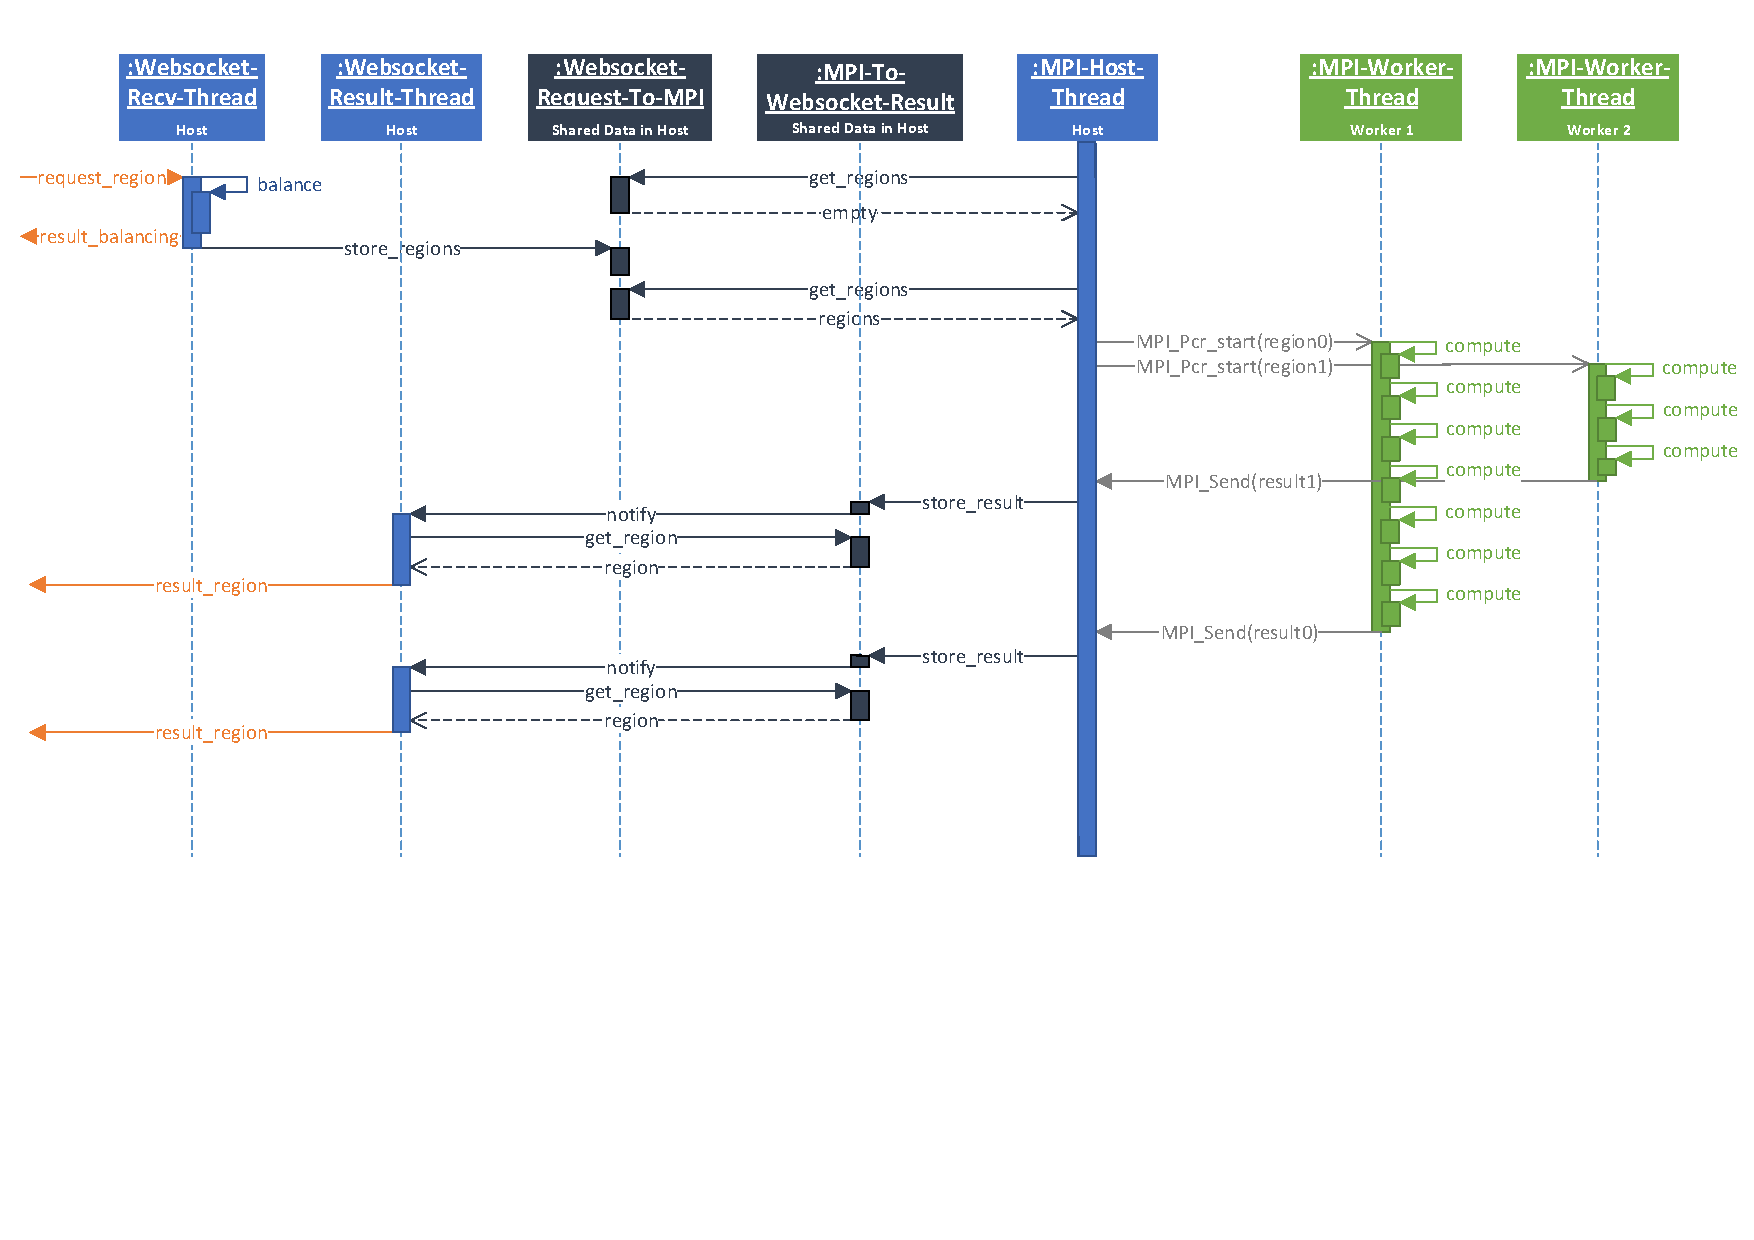
\includegraphics[angle = 90, origin = c, trim = 0mm 0mm 80mm 0mm, clip, width=0.98\linewidth]{img/Implementierung/MPISequenzdiagrammFarben.pdf}
	\caption{Sequenzdiagramm zur Kommunikation im Backend}
	\label{fig:mpi_sequenzdiagramm}
\end{figure}

Der MPI-Thread des Hosts erwartet in einer mit dem Websocketthread geteilten Datenstruktur
Rechenaufträge, die per MPI an die Worker weiter geleitet werden sollen.
Diese führen die zugewiesenen Rechenaufträge gegebenenfalls mithilfe von SIMD und / oder OpenMP parallelisiert aus.
Anschließend werden die Rechenergebnisse wieder via MPI an den MPI-Thread übermittelt,
welcher diese in einer weiteren gemeinsamen Datenstruktur ablegt.

Der Ablauf dieser Kommunikation wird in \autoref{fig:mpi_sequenzdiagramm} veranschaulicht.

Wird während einer laufenden Berechnung eine neue Berechnung angefordert, so werden die auf den Workern noch laufenden Berechnungen abgebrochen und mit der neuen Berechnung begonnen. Ein entsprechendes Sequenzdiagramm ist im Anhang (TODO Link) zu finden.

Da mehrere Threads in der Host-Anwendung für die Websocketfunktionalität unumgänglich sind sollte bei dem System
auf dem das Program laufen soll darauf geachtet werden, dass die lokale MPI-Implementierung das Threadlevel \verb|MPI_THREAD_FUNNELED| unterstützt.

\subsubsection{MPI-Designentscheidungen}
%TODO Namen der Threads überall (auch Grafiken) konsistent halten! Sollte aktuell passen. Vor der Abgabe nochmal überprüfen.
Für die Implementierung der MPI-Kommunikation wurden zur Performanzsteigerung folgende Designentscheidungen getroffen:

\begin{itemize}

	\item \label{item:mpi_init} Initialisierung der MPI-Umgebung mit MPI\_THREAD\_FUNNELED

          In der gewählten Architektur arbeiten sowohl Host als auch Worker mit mehreren Threads, wobei nur der Hauptthread MPI-Aufrufe tätigt.
          Für die MPI-Konfiguration bedeutet dies, dass sie mit MPI\_THREAD\_FUNNELED initialisiert werden muss.
          Durch die Beschränkung auf einen MPI-Thread werden MPI-Seitig Optimierunge ermöglicht.
          Es wurde sich bewusst gegen den Einsatz von MPI in mehreren Threads (MPI\_THREAD\_MULTIPLE) entschieden, da OpenMPI hierfür zwar eine korrekte aber nicht performanceoptimierte Implementierung anbietet \footnote{siehe Abschnitt 'MPI\_THREAD\_MULTIPLE Support' unter \url{https://www.open-mpi.org/doc/v3.1/man3/MPI_Init_thread.3.php}}.

	\item Datenübertragung als uninterpretierte Byte-Datenströme

          Alle per MPI übertragenen Daten werden uninterpretiert als Byte-Datenströme geschickt.
          Das bedeutet, dass die Interpretation der Daten Maschinenabhängig ist.
          Allerdings macht dies die Übertragung einfach und performant, da im gesamten Backend mit den selben Structs ohne eine Umformatierung gearbeitet werden kann.

	\item Nicht-blockierendes Senden der Subregionen vom Host an die Worker

          Der MPI-Host-Thread verwendet Persistent Communication Requests für das performante Senden der Arbeitsaufträge zu den Workern,
          da hier die Nachrichtengröße konstant ist und die Sendeparameter identisch sind.
          Die Übertragung wird nicht-blockierend durchgeführt,
          sodass alle Sendeoperationen parallel starten und anschließend auf deren Abschluss mit einem MPI\_Waitall() zu warten.
          Dieser Aufruf ist in der Grafik mit "MPI\_PCR\_Start()" bezeichnet.

	\item Nicht-blockierendes Empfangen der vom Host gesendeten Subregionen in den Workern

          Analog zum MPI-Host-Thread nutzt auch der MPI-Worker-Thread Persistent Communication Requests um eine Subregion
          mit möglichst wenig Overhead, zu empfangen.
          Es wurde der nicht-blockierende Übertragungsmodus gewählt, um laufende Berechnungen abbrechen zu können,
          sobald ein neuer Rechenauftrag empfangen wird (siehe \hyperref[para:impl_mpi_worker]{Implementierung der MPI-Kommunikation im Worker}).

	\item Struktur der von den Workern an den Host gesendeten Daten

          Es müssen generelle Informationen in Form eines WorkerInfo-Structs (allgemeine Daten zur Subregion, Nummer des Workers, Berechnungsdauer) und ein Array der berechneten Daten von den Workern an den Host gesendet werden.
          Da die Anzahl der berechneten Daten und damit die Länge des Datenarrays variiert, wird das Datenarray direkt hinter das WorkerInfo-Struct kopiert und zusammen versendet.

	\item Blockierendes Senden der berechneten Subregion von den Workern an den Host

          Nicht-blockierendes Senden ist hier nicht notwendig, da nach der abgeschlossenen Berechnung neben dem Senden keine weiteren Operationen durchzuführen sind.
          Im Sequenzdiagramm ist dieser Aufruf mit "MPI\_Send()" bezeichnet.

	\item Blockierendes Empfangen der von den Workern berechneten Subregionen im Host

          Wenn ein Worker Daten zum Versenden bereit hält (dies wird nicht-blockierend mit MPI\_Iprobe() getestet), werden die Daten blockierend Empfangen und sofort im richtigen Format in die MPI\_To\_Websocket\_Result Datenstruktur abgelegt.

	\item Busy Waiting

	      \begin{itemize}
		      \item Busy waiting im MPI-Host-Thread

		            Im Host ist busy waiting unumgänglich, da einerseits auf neue Arbeitsaufträge und andererseits auf Rechenergebnisse reagiert werden muss. Um busy waiting zu umgehen, wäre eine Lösung, einen Sendethread und einen Empfangsthread zu implementieren, was aber die MPI-Kommunikation insgesamt verlangsamen würde, da ein höherer Isolation-Level gesetzt werden muss (siehe \hyperref[item:mpi_init]{Initialisierung der MPI-Umgebung mit MPI\_THREAD\_FUNNELED}). Um die CPU zu entlasten, wird der MPI-Host-Thread für 100 Mikrosekunden schlafen gelegt, falls im aktuellen Schleifendurchlauf weder eine Sendeoperation noch eine Empfangsoperation durchgeführt wurde. Diese Pause hat keine signifikante Auswirkung auf die Gesamtperformance aufgrund der im Vergleich deutlich längeren Berechnungsdauer einer Subregion.
		            %TODO Evtl. nicht-blockierend mit Sendeoperation daweil starten

		      \item Busy waiting im MPI-Worker-Thread

                    Solange keine Berechnungen durchzuführen sind, wäre es ausreichend blockierend auf das Eintreffen neuer Berechnungsaufträge zu warten, um die CPU nicht unnötig zu belasten.
                    Da die blockierende Empfangsoperation MPI\_Recv() jedoch häufig selbst mit busy waiting implementiert ist, wird auf deren Nutzung verzichtet. Stattdessen wird der MPI-Worker-Thread im Schleifendurchlauf für 1 Millisekunde schlafen gelegt wenn keine Nachrichten zu empfangen sind. Im Vergleich zur Berechnungsdauer einer Subregion fällt diese 1 Millisekunde nicht ins Gewicht, entlastet aber spürbar die CPU.
		            %TODO Quellen für den Busy Waiting Dreck.

	      \end{itemize}

\end{itemize}

\subsubsection{MPI-Kommunikation im Host}

%TODO Eventuell noch das Senden der Testregionen beschreiben.
Die Kommunikation zwischen Host (MPI-Host-Thread) und Workern (MPI-Worker-Thread) ist im MPI-Host-Thread als Endlosschleife (busy waiting) implementiert. Die dabei stattfindenden Operationen inklusive ausführlicher Kommentare sind in \autoref{src:mpi_host_pseudo} einzusehen.

\begin{figure}[!h]
	\lstinputlisting[language=python, caption={MPI Kommunikation im Host in Pseudocode}, label={src:mpi_host_pseudo}]{code/MPIHost.py}
\end{figure}

\subsubsection{Ablauf der MPI-Kommunikation im Worker}\label{para:impl_mpi_worker}

Analog zum Host ist auch der Worker (MPI-Worker-Thread) als Endlosschleife mit busy waiting implementiert. Die Berechnung einer Subregion erfolgt dabei zeilenweise durch einen compute() Aufruf. Der entsprechende Pseudocode inklusive ausführlicher Kommentare ist in \autoref{src:mpi_worker_pseudo} zu finden.

\begin{figure}[!h]
	\lstinputlisting[language=python, caption={MPI Kommunikation im Worker in Pseudocode}, label={src:mpi_worker_pseudo}]{code/MPIWorker.py}
\end{figure}


\subsection{Berechnung der Mandelbrotmenge}\label{sec:mandelbrot_calculation}

Die Berechnung der einzelnen Punkte der Mandelbrotmenge ist in eine eigene Klasse ausgelagert.
Wie bei der \hyperref[sec:load_balancing]{Lastbalancierung} sind die Klassen nach dem Strategy-Pattern strukturiert, um eine spätere Erweiterung um andere Fraktale zu vereinfachen.
Das Interface der Strategien ist hier in der Klasse \verb|Fractal| definiert.

Zusätzlich beinhaltet \verb|Fractal| statische Methoden zur Berechnung der Deltas für Real- und Imaginärteil.
Diese geben die Größe des Bereichs der komplexen Ebene an, der von einem Pixel überdeckt wird.
So berechnet sich zum Beispiel das reelle Delta wie folgt:

\begin{equation*}
	deltaReal = \frac{maxReal - minReal}{width}
\end{equation*}

Die Berechnung des imaginären Deltas erfolgt analog.
Die Deltas werden u.a. für die Berechnung des Fraktals in den Workern verwendet.

\subsubsection{Berechnung ohne SIMD}

Die Klasse \verb|Mandelbrot| stellt die Methode \verb|calculate_fractal| bereit,
die für ein übergebenes Array an Punkten die Iterationszahl bestimmt.
Diese Übergabemethode macht ein gemeinsames Interface mit den \hyperref[subsec:simd]{vektorisierten Versionen} möglich.

Die Berechnung eines Punktes ist nun nicht weiter schwer, es muss lediglich \autoref{equ:mandelbrot} als C++-Code umgesetzt werden.
Bei $|z_n| > 2$ die Berechnung abgebrochen werden, da der Punkt sicher nicht in der Mandelbrotmenge liegt.
Um Rechenzeit zu sparen wird dabei in allen Implementierungen die äquivalente Formel $Re(z_n)^2 + Im(z_n)^2 > 4$ evaluiert.
Die Berechnung wird ebenfalls abgebrochen, wenn die maximale Anzahl an Iterationen erreicht wurde.
Die benötigte Anzahl an Iterationen wird in ein übergebenes Array geschrieben.

\subsubsection{Berechnung mithilfe von SIMD}\label{subsec:simd}

Um das Parallelisierungskonzept mithilfe von SIMD zu erklären,
ist es hilfreich zunächst vor Augen zu führen, wie ein Vektor komplexer Koordinaten ohne SIMD verarbeitet würde,
sodass die Schleife über den Vektor parallel ausgeführt werden kann.
Für SIMD ist wichtig dass dabei die einzelnen Rechenschritte synchron stattfinden können,
damit die verschiedenen Werte mit ein und derselben Instruktion verarbeitet wird.
Dies ist in \autoref{src:MandelbrotVect} zu sehen.
Die Berechnung der einzelnen Kooridnaten bleibt gleich, nur die Abbruchbedingung wird auf alle bearbeiteten Koordinaten erweitert.

Es muss also solange weiter iteriert werden, bis für alle Komponenten die Berechnung abgebrochen werden darf.
Hierbei ist es kein Problem mit den abgebrochenen Punkten weiter zu rechnen, sofern die
Iterationszahl nur hochgezählt wird wenn das $z_n$ der Koordinate Betragsmäßig kleiner gleich $2$ ist.
Dies gilt, da alle $|z_{n+i}| > 2$ sofern $|z_n| > 2$ \cite{424331}.

Außerdem ist zu beachten, dass die Iterationszahl vor der Berechnung der nächsten Iteration erhöht werden muss.
Dies liegt darin begründet, dass die Iterationszahl die Anzahl der Rechenschritte repräsentieren soll und
der nächste Schritt sicher ausgeführt wird.
Auch dann, wenn in auf Basis der neuen Berechnung bereits abgebrochen würde.

\begin{figure}[h!]
	\lstinputlisting[caption={Bearbeitung eines Vektors komplexer Koordinaten in Pseudocode}, label={src:MandelbrotVect}]{code/mandelbrotvect.pseudo}
\end{figure}

Für ARMv8-Architektur-Prozessoren wie die Prozessoren des Raspberry Pi 3 B+ oder ODroid
existieren zur Implementierung von SIMD Instruktionen in Hochsprachen wie C und C++ sogenannte
NEON Compiler Intrinsics\footnote{Details im Abschnitt \enquote{Compiler Intrinsics} unter \url{https://developer.arm.com/technologies/neon}}.

Diese Intrinsics ermöglichen eine Verwendung der nativen SIMD-Befehle, wobei der Compiler sich um die Verwendung der SIMD-Register kümmert.
Dadurch wird lesbarer Code ermöglicht, der sich stärker am zu implementierenden Algorithmus orientiert.

Zu den hier benötigten mathematischen Operationen (z.B. der Addition) wird hierbei das Compiler Intrinsic nach folgendem Schema erzeugt:
\texttt{v\textit{opc}q\_f\textit{pr}} mit dem Operationscode \textit{opc} (z.B. \textit{add} für Addition).
\verb|v| ist das allgemeine Prefix für Vektoroperationen und \verb|q| bedeutet, dass doppelt so viele Register verwendet werden wie ohne \enquote{q}.
Das Postfix f\textit{pr} bestimmt, dass die Register als Gleitkommazahlen der Präzision \textit{pr} bit (in diesem Fall 32 oder 64) interpretiert werden sollen.
Damit werden in jeder Operation 4 mal 32 bit Gleitkommazahlen oder 2 mal 64 bit Gleitkommazahlen verrechnet.

Mithilfe der in SIMD-Intrinsics ist die Umsetzung dieses Codes sehr direkt möglich.
Bei der Hardware-beschleunigten Variante mit SIMD, wurde stets das Postfix \verb|q| eingebunden.
Damit werden alle verfügbaren SIMD-Register des ARMv8-A Prozessors des ODroids und Raspberry Pi 3 B+ herangezogen.

Zusätzlich wurden Optimierungen mithilfe der NEON-nativen multiply-add (\textit{mla}) und multiply-subtract (\textit{mls}) Befehle vorgenommen.
Zudem kann der parallele Vergleich zweier Vektoren (\textit{clt}) ausgenutzt werden, wobei als Ergebnis jedoch nicht 1 und 0 ausgegeben werden,
sondern alle Bits der Ergebnisvektorkomponente auf 1 gesetzt werden sofern die Bedingung erfüllt ist und sonst auf 0.
Um im weiteren Verlauf effizient die Vektorkomponenten aufzuaddieren (\textit{addv}) wird die ursprünglich vorzeichenlose Zahl als vorzeichenbehaftet interpretiert.
Jede Komponente für die die Bedingung zu wahr evaluiert hat, kann nun als $-1$ interpretiert werden.
Die Summe über die Komponenten entspricht damit der negierten Anzahl an noch nicht abgeschlossenen Punkten.

\subsection{Leistungssteigerung durch Parallelisierung auf Thread Level mithilfe von OpenMP}

\verb|OpenMP|\footnote{\url{https://www.openmp.org/wp-content/uploads/openmp-4.5.pdf}} (Open Multi-Processing) ist ein API, das auf die Parallelisierung von Schleifen und Programmabschnitten auf Shared Memory Systemen spezialisiert ist. Parallel ausführbare Programmteile werden durch eine spezielle Präprozessor Anweisung für die parallele Ausführung in mehreren Threads gekennzeichnet.
\\ \\
Bei der Berechnung der Mandelbrotmenge wird OpenMP im Worker verwendet um die for-Berechnungsschleife parallel auf den zur Verfügung stehenden Threads auszuführen. Dies dient dazu, die Leistung des Workers signifikant zu steigern. Die dabei genutzte Anweisung setzt sich folgendermaßen zusammen:

\begin{itemize}
	\item \verb|#pragma omp parallel for| kennzeichnet die darauf folgende for-Schleife für die parallele Ausführung.
\end{itemize}

Folgende Parameter werden dabei noch gesetzt:

\begin{itemize}
	\item \verb|shared(<Datenstrukturen>)| kennzeichnet diejenigen Datenstrukturen die parallel beschreibbar sind.

	\item \verb|schedule(<Parameter>)| setzt die gewählte Schedulingstrategie fest. Als Parameter wurde genutzt:

	      \begin{itemize}
		      \item \verb|nonmonotonic| besagt, dass die Schleifeniterationen in beliebiger Reihenfolge ausgeführt werden können.

		      \item \verb|dynamic, 10| bedeutet, dass jeder Thread zunächst 10 Schleifeniterationen zur Berechnung zugewiesen bekommt. Hat ein Thread diese Aufgabe abgeschlossen, bekommt er weitere 10 Iterationen falls noch welche verfügbar sind. Diese Strategie wurde gewählt, um die Rechenlast möglichst gleichmäßig auf alle Threads zu verteilen und so die Gesamtrechenzeit der Schleife zu minimieren ohne eine erneute Lastbalancierung vornehmen zu müssen.
	      \end{itemize}
\end{itemize}


\subsection{Websocketverbindung}\label{cls:Host}

Direkt nach der Initialisierung des Host-Programms wird ein separater Thread gestartet, der über Websocket
Anfragen zur Berechnung einer Region entgegennimmt sowie ein Thread, der berechnete Regionen an den verbundenen Client übergibt.
%Die Methode \verb|Host::start_server| initialisiert dabei lediglich den Websocketserver.
%Über den Typ des Servers wird eine Kompression versendeter Nachrichten über die im Standart akzeptierte Extension \enquote{perMessageDeflate} aktiviert.
Der Websocketserver wird mit \verb|server.init_asio()| mit der Transport Policy "transport::asio"
konfiguriert, sodass Multithreadzugriffe auf Sende- und Empfangsmethoden problemlos möglich sind \cite{websocketppManual}.

Es sollte beachtet werden, dass der Server zu jedem Zeitpunkt lediglich die zuletzt geöffnete Verbindung speichert.
Nachrichten vom Frontend werden mit der Methode \hyperref[cls:Host::handle_region_request]{\texttt{Host::handle\_region\_request}} entgegengenommen.
Der zweite bei der Initialisierung gestartete Thread führt die Methode \hyperref[cls:Host::send]{\texttt{Host::send}} aus, die Nachrichten zurücksendet.

Die entstehende Dynamik kann dem Sequenzdiagramm \autoref{fig:mpi_sequenzdiagramm} entnommen werden.

\paragraph{Host::handle\_region\_request}\label{cls:Host::handle_region_request}

Die Methode dekodiert einen empfangene Nachricht als JSON Regionsanfrage und behandelt sie nach folgendem Schema:

\begin{enumerate}
	\item Parse das empfangene RegionRequest-Objekt. Bei Fehlern wird die Funktion abgebrochen.
	\item Involviere den spezifizierten Lastbalancierer um eine Aufteilung der Region zu erhalten
	\item Bestimme den Rang des Workers, der eine Region bearbeiten wird. Hierzu wird der Algorithmus aus \autoref{src:Host.cpp.handle_region_request} verwendet.
	\item Sende die Aufteilung inklusive der Ränge aller beteiligten Worker als Regions-Objekt an das Frontend
	\item Übergebe die aufgeteilten Regionen über eine geteilte Datenstrukutr an den MPI-Thread, der diese an die Worker sendet.
\end{enumerate}

In dem JSON wird unter dem Schlüssel \texttt{"balancer"} ein String erwartet, der den zu wählenden Lastbalancierer bestimmt.
Mögliche Zeichenketten hierfür sind in den Klassen der Balancierer unter \verb|backend/src/balancer| in der globalen Variable
\verb|Klassenname::NAME| gespeichert.

Es ist hierbei wichtig, dass das Senden an die Worker erst nach der Antwort an das Frontend geschieht und wird daher garantiert.
Dadurch kann im Frontend sichergestellt sein, dass alle eintreffenden RegionData-Objekte zu einer Regionsaufteilung gehören,
die bereits empfangen wurde.

\paragraph{Host::send}\label{cls:Host::send}

Während ein Thread das Empfangen von Nachrichten übernimmt, behandelt diese Methode von den Workern fertig berechnete Regionen.
Die Methode setzt dabei eine Dauerschleife nach folgendem Schema um:

\begin{enumerate}
	\item Überprüfe auf das Vorhandensein fertig berechneter Regionen \label{enum:Host::send.step1}
	\item Ist keine Region verfügbar
	      \begin{enumerate}
		      \item Warte blockierend auf eine Änderung
		      \item Springe zu Schritt \ref{enum:Host::send.step1}
	      \end{enumerate}
	\item Ist eine Region verfügbar
	      \begin{enumerate}
		      \item Locke die geteilte Datenstruktur
		      \item Entnimm eine Region daraus
		      \item Löse das Lock
	      \end{enumerate}
	\item Codiere die Regionsdaten in JSON und versende sie über Websocket an den aktuell verbundenen Client
	\item Springe anschließend zu Schritt \ref{enum:Host::send.step1}
\end{enumerate}

Ein Beispiel für versendete Regionsdaten kann \autoref{src:regionData.json} entnommen werden.

Mithilfe einer \texttt{condition\_variable}\footnote{\url{https://en.cppreference.com/w/cpp/thread/condition_variable}}
nutzt sie die C++11 nativen mutex-Mechanismen um über das Vorhandensein neuer Regionen informiert zu werden.

\subsection{Implementierung des Frontends}
\begin{figure}
	\centering
	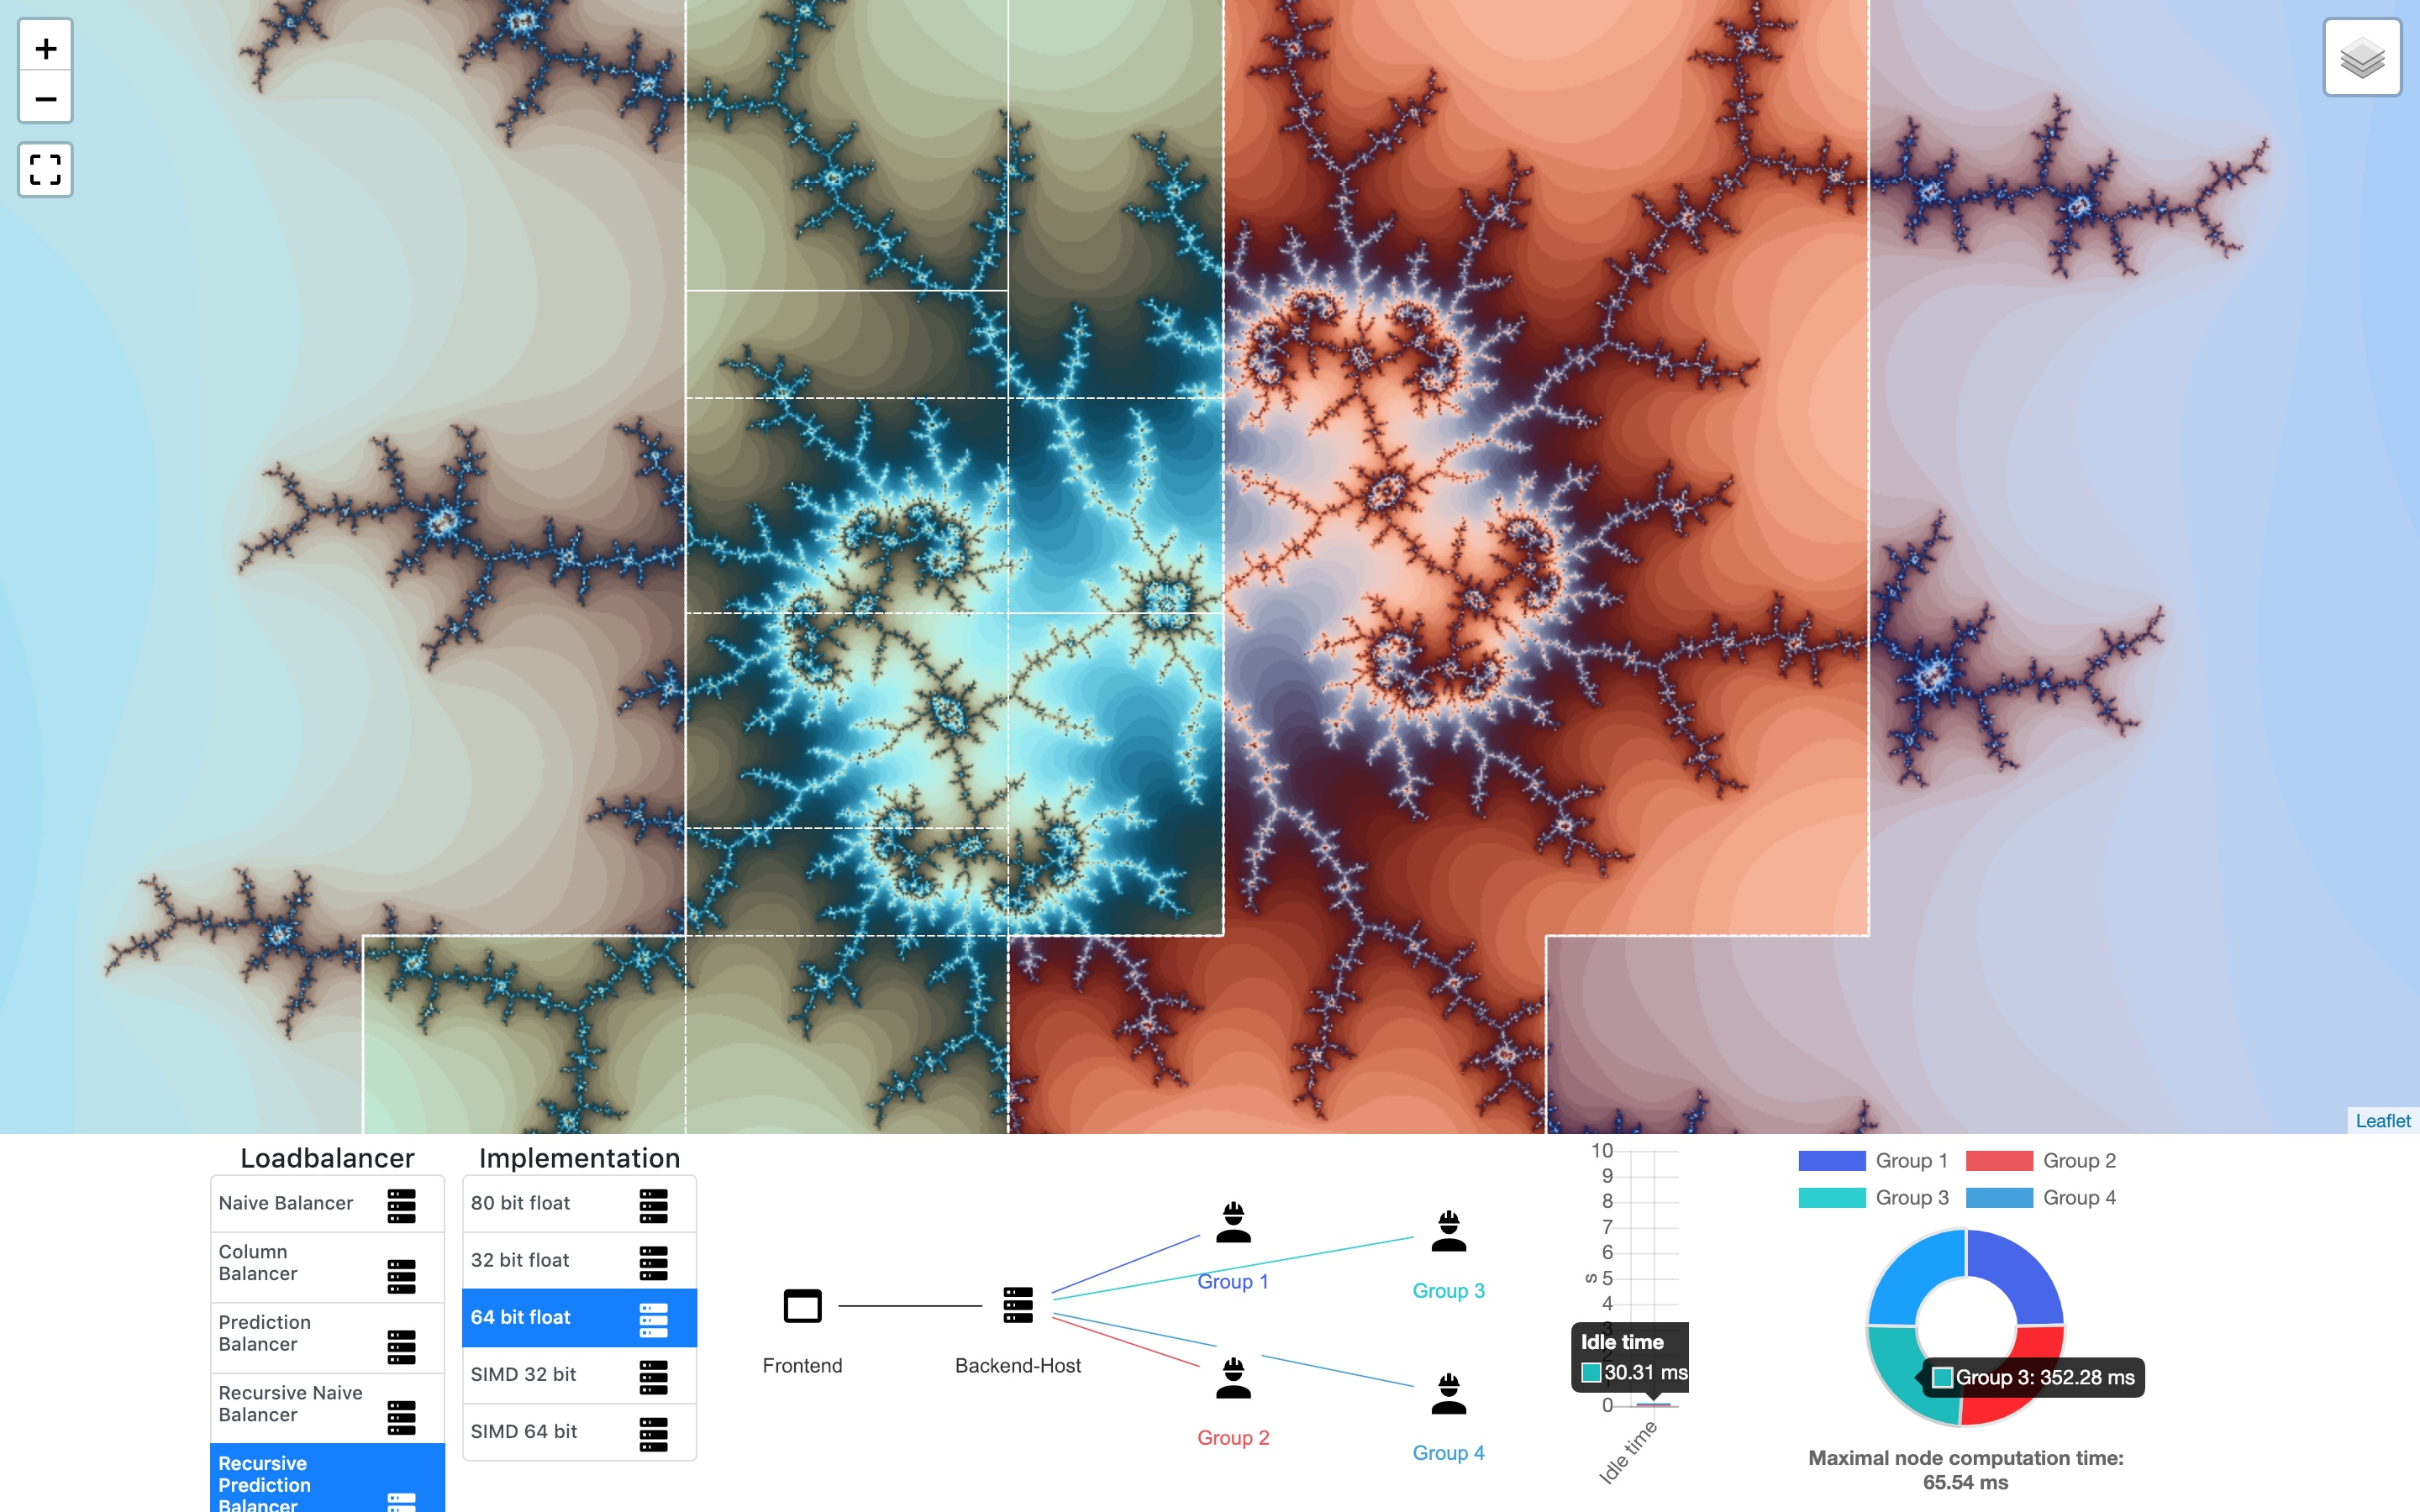
\includegraphics[width=\linewidth]{img/Implementierung/ui}
	\caption{Benutzeroberfläche der Mandelbrot Anwendung}
	\label{fig:ui-screenshot}
\end{figure}
Um das Frontend zu implementieren, wurde sich für die Programmiersprache TypeScript\footnote{\url{https://www.typescriptlang.org/}}(Erweiterung von JavaScript um Typisierung) entschieden.
Da diese zu JavaScript kompiliert, werden die Vortele von JavaScript, wie Ausführung im Webbrowser des Benutzers und eine vielzahl verfügbarer Bibliotheken,
mit den Vorteilen einer typisierten Programmiersprache vereint.


Für die graphische Benutzeroberfläche wurde ebenfalls TypeScript mit dem React Framework\footnote{\url{https://reactjs.org/}} verwendet, welches es ermöglicht,
graphische Komponenten nativ in TypeScript zu erstellen und dynamisch zu verändern.
Es wurde für jede Komponente eine eigene TypeScript Klasse zu erstellt, welche dann den betreffenden
das betreffende Verhalten und dessen Darstellung enthält.


Um das Fraktal darzustellen wird die Leaflet\footnote{\url{https://leafletjs.com/}} Bibliothek verwendet.
Diese, für Onlinekarten konzipierte, Bibliothek stellt den Bereich der komplexen Ebene, auf der die Mandelbrotmenge liegt dar.
Dabei wird der momentan sichtbare Ausschnitt der Menge mit Hilfe der WebSockets Verbindung (siehe \autoref{sec:fontend_communication}) an das Backend versendet und vom ausgewählten Lastbalancierer in Teilregionen unterteilt (siehe \autoref{sec:load_balancing}).
Jeder der vom Backend berechneten Teilregionen wird, sobald diese empfangen wurden, im Frontend angezeigt und die Komponenten
zu Visualisierung der Rechenzeit aktualisiert.

\subsubsection{Kommunikation mit dem Backend}\label{sec:fontend_communication}
Zur Kommunikation mit dem Backend wird im Frontend ein Objekt der Klasse \verb|WebSocketClient| erzeugt.
Alle zur Verbindung mit dem Backend verwendeten Codestücke liegen dabei in dem Ordner \verb|src/connection/|.

Die dort definierte Klasse \verb|WebSocketClient| abstrahiert von dem JavaScript-nativen Websocketinterface \verb|WebSocket|\footnote{\url{https://developer.mozilla.org/en-US/docs/Web/API/WebSocket}}.
Bei der Initialisierung baut das erzeugte Objekt eine Verbindung zu der lokalen Adresse \url{ws://localhost:9002} auf\footnote{
	Faktisch wird eine Verbindung geöffnet, geschlossen und erneut geöffnet.
	Dies ist durch ein ungelöstes Problem beim Verbindungsaufbau bedingt, das dafür sorgt, dass ein Verbindungsaufbau
	erst bei der zweiten erzeugten Websocketverbindung fehlerfrei gelingt.
}.
Dort muss das Backend bereit sein, eine Websocketverbindung anzunehmen.

Die Klasse \verb|WebSocketClient| bietet dabei folgende Methoden:
\begin{itemize}
	\item \verb|sendRequest(request)|

	      Diese Methode versendet das übergebene RegionRequest-Objekt codiert als \verb|JSON|\footnote{\url{https://www.json.org/}}-Objekt an das Backend.
	\item \verb|registerRegion(fun), registerRegionData(fun)|

	      An diese Methoden können Callbacks übergeben werden, die aufgerufen werden, wenn das Frontend über die Websocketverbindung
	      respektive ein \texttt{Region}-Objekt oder ein \texttt{RegionData}-Objekt empfängt.
	      Diese sind die Aufteilung einer angefragten Region (siehe \autoref{src:region.json})
	      oder die berechneten Iterationswerte einer Region (siehe \autoref{src:regionData.json}).

	      Die übergebenen Callbacks erhalten als Parameter respektive die vorgruppierte Aufteilung als ein Array von Workergruppen (\texttt{RegionGroup})
	      oder das \verb|JSON|-dekodierte \verb|RegionData|-Objekt.
\end{itemize}
Zudem wird hierbei bereits eine Filterung der eingehenden Regionsdaten vorgenommen.
Bei Empfang einer Regionsaufteilung, wird diese zwischengespeichert.
Jedes empfangene Regionsdatenobjekt wird dann bei Empfang daraufhin überprüft,
ob der darin dargestellte Ausschnitt einer Regionsaufteilung entspricht (dazu wird das \verb|region|-Attribut verglichen)
und das dargestellte Fraktal der zuletzt übergebenen Auswahl entspricht.
Diese Filtrierung ist notwendig, da Worker Regionsdaten auch \enquote{verspätet} absenden können,
falls bei dem zuvorgehenden Bereich nicht gewartet wurde bis die Berechnungen aller Worker entgegengenommen wurden.
Die Definitionen der zugehörigen Objekt-Interfaces finden sich in den Dateien \verb|RegionGroup.ts| und \verb|ExchangeTypes.ts| finden.

Anfragen an das Backend werden dabei mit der folgenden Funktion in \verb|RegionRequest.ts| erstellt:
\begin{itemize}
	\item \verb|request(map, balancer, implementation)|:
	      Diese extrahiert aus der übergebenen Sicht auf die Mandelbrotmenge, die in der Leaflet-Karte gespeichert ist,
	      die Parameter zum Anfragen einer Region.
	      Dazu werden mithilfe des aktuellen Zooms der linke obere und rechte untere Punkt des Sichtbereiches
	      in dem Leaflet-internen Koordinatensystem auf entsprechende Punkte in der komplexen Ebene projeziert.
	      Da zum Erzeugen des passenden Objektes auch der gewünschte Lastbalancierer und der Fraktaltyp notwendig sind,
	      werden diese als weitere Parameter übergeben.

	      Die Funktion gibt direkt ein Objekt zurück, dass das Interface \verb|RegionRequest| erfüllt.
\end{itemize}

\subsubsection{Darstellung der Regionsdaten} % tileDisplay/

Die für die Darstellung der Mandelbrotmenge verwendete Bibliothek (leaflet) hat die Einschränkung, dass
nur Quadrate einer vordefinierten Größe (\verb|Tiles|) angezeigt werden können. Ebenfalls verwendet diese ein
eigenes Koordinatensystem, unter welchem jede angezeigte Tile eindeutig mit dem Tripel \( (x, y, zoom) \)
identifiziert wird. Somit ist eine Übersetzung zwischen den Daten des Backends und den von leaflet erwarteten nötig.

\paragraph{MatrixView.ts, RegionOfInterest.ts}\label{par:matrixView}
Die Klasse \verb|MatrixView.ts| implementiert die Umsetzung einer vom Backend versendeten Region zu
den von leaflet erwarteten Tiles.
\begin{itemize}
	\item \verb|registerTile(point, draw)|

	      Alle sichtbaren Tiles registrieren sich mit dem Callback \verb|draw|,
	      welcher ausgeführt wird, sobald die anzuzeigenden Daten für die
	      entsprechende Tile verfügbar sind. Diese Iterationswerte des Backends werden dabei der \verb|draw| Funktion als Parameter
	      in Form eines \verb|RegionOfInterest| Objekts übergeben.
\end{itemize}


Ein \verb|RegionOfInterest| Objekt implementiert wiederum die Übersetzung von lokalen \( (x,y) \) Pixel-Werten
einer Tile zu Indizes in das vom Backend gesendete Array an Regionsdaten (siehe \autoref{src:regionData.json}).
\begin{itemize}
	\item \verb|get(x, y)|

	      Gibt, für einen Tile \( (x,y) \) Pixel-Wert die benötigte Iterationsanzahl zurück.
	      %   (siehe \autoref{src:RegionOfInterest.ts}).
	      %   \begin{figure}[h!]
	      %       \lstinputlisting[caption={Umsetzung von Pixel-Werten der Tiles zu Indizes in Regionsdaten}, label={src:RegionOfInterest.ts}, language=TypeScript, firstline=41, lastline=48, firstnumber=41]{../../frontend/src/tileDisplay/RegionOfInterest.ts}
	      %   \end{figure}
\end{itemize}


\paragraph{TileDisplay.tsx}
Die Klasse \verb|TileDisplay.tsx| verwendet die leaflet Bibliothek direkt, um die Regionsdaten darzustellen.
Dabei wird dieser die WebSocket Verbindung in Form eines \verb|WebSocketClient|, sowie der vom Nutzer gewählte Balancer,
die Implementierung und Gruppierung durch \verb|Observable| Klassen (siehe \autoref{par:observables}) übergeben. Ebenfalls wird der anzuzeigende Ausschnitt der
Mandelbrotmenge übergeben.

Da das Backend die berechneten Teilbereiche der Mandelbrotmenge als Regionen zurück gibt, dessen Höhe und Breite
Vielfache der leaflet Tile-Größe sind, wird eine Region dem Benutzer durch mehrere Tiles dargestellt.
Dieses Verhältnis wird in \autoref{fig:leafletTiles} dargestellt.

\begin{figure}
	\centering
	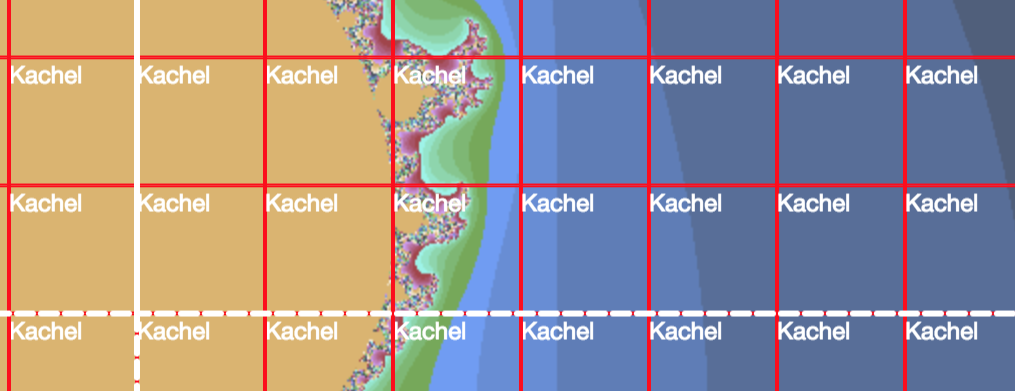
\includegraphics[width=0.5\linewidth]{img/Implementierung/leafletTiles}
	\caption{Relation von Backend Regionen zu leaflet Tiles (Kachel).
		Dabei ist beispielhaft eine Region des Backends
		weiß eingezeichnet, alle leaflet Tiles sind rot umrandet angegeben.
	}\label{fig:leafletTiles}
\end{figure}

Zudem ist die Darstellung der Iterationswerte, sowie Regionsaufteilung durch unterschiedlichen Ebenen innerhalb der
leaflet Bibliothek realisiert:

\begin{itemize}
	\item \verb|MandelbrotLayer| in \verb|TileDisplay.tsx|

	      In dieser eigenen Ebene der leaflet karte werden die Tiles dargestellt.
	      Dieser erstellt für den sichtbaren Bereich\footnote{
		      Da die Fenstergröße des sichtbaren Bereichs keien Vielfaches der Tilegröße sein muss,
		      können Tiles erzeugt werden, welche teilweise außerhalb des sichtbaren Beriechs liegen}
	      alle benötigten Tiles. Für jede der Tiles wird ein \verb|HTML5 canvas|\footnote{\url{https://developer.mozilla.org/kab/docs/Web/API/Canvas_API}} Objekt erstellt, welches es
	      ermöglicht, für jeden Pixel einen \( (r,g,b) \) Farbwert zu definierten und anzuzeigen. Wobei die Farbwerte aus den berechneten
	      Iterationswerten des Backends mit einem Shader (siehe \autoref{par:shader}) ermittelt werden. Die Iterationswerte können wiederum
	      mit einem \verb|MatrixView| Objekt aus den Regionsdaten des Backends gelesen werden.

	\item \verb|WorkerLayer| in \verb|WorkerLayer.ts|\label{par:workerLayer}

	      Diese Klasse visualisiert die Regionsaufteilung des Lastbalancierers als Overlay, welche über den Iterationswerten
	      dem Benutzer angezeigt wird.
	      Dafür wir eine in leaflet bestehende \verb|GeoJSON| API verwendet, mit welcher es möglich
	      ist, beliebige Polygone auf den bestehenden Kartendaten anzuzeigen. Die Knoten dieser Polygone werden dabei jede \verb|RegionGroup|
	      mit Hilfe der Funktionen aus \verb|Project| von Koordinaten der komplexen Ebene, welche im Backend verwendet werden, zu
	      leaflet Koordinaten umgerechnet.

	      \begin{figure}
		      \centering
		      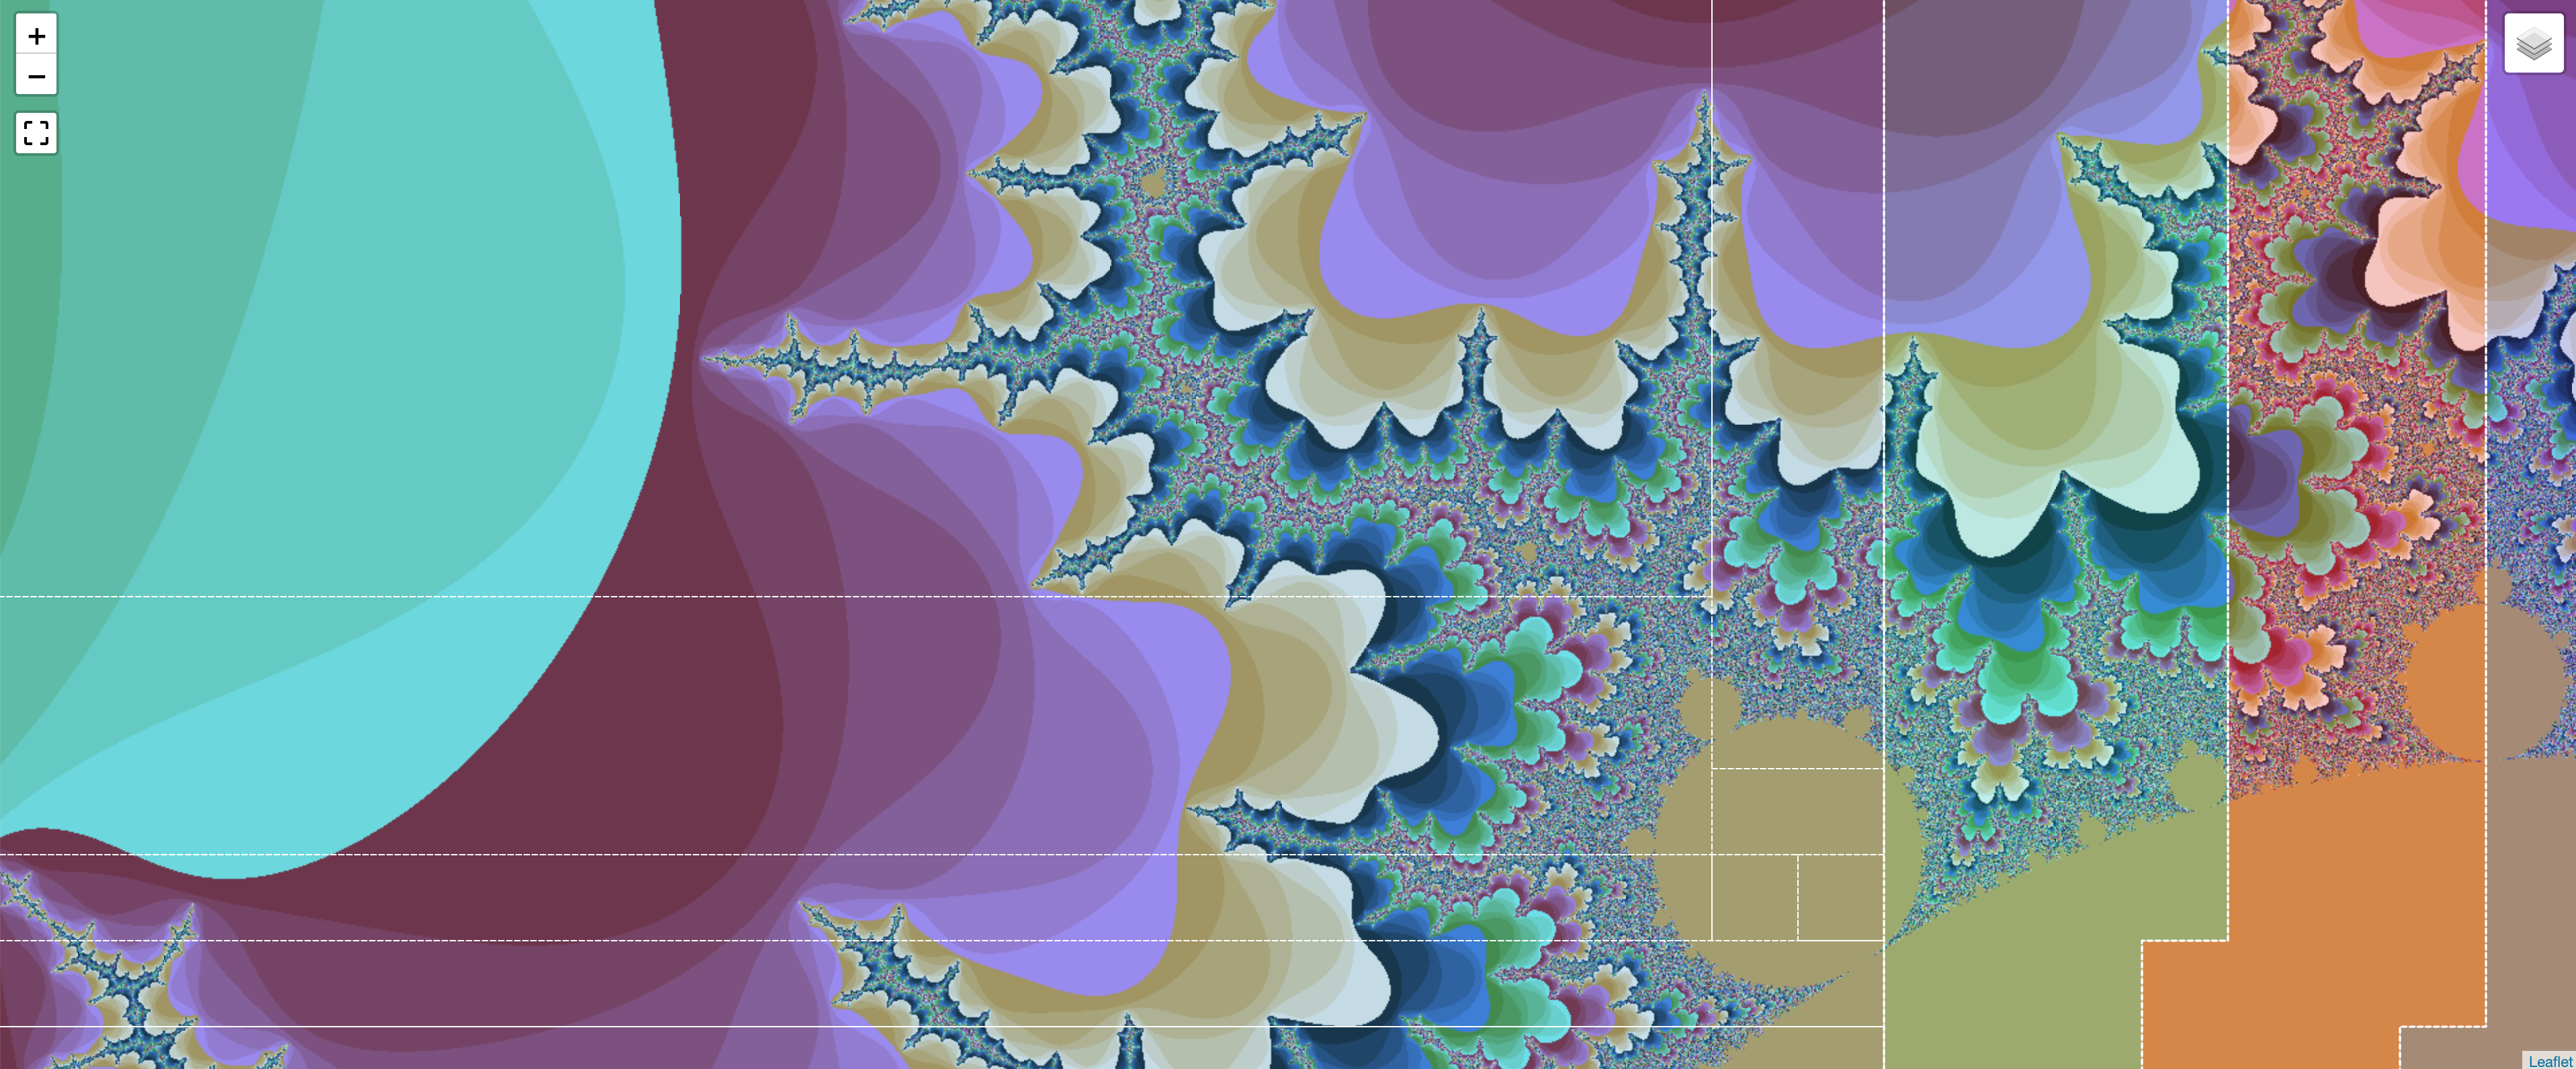
\includegraphics[width=.85\linewidth]{img/Implementierung/regionGrouping}
		      \caption{WorkerLayer für eine Gruppierung der Aufteilung des Recursive PredictionBalancers mit 37 Workern}
		      \label{fig:regionGrouping}
	      \end{figure}

	      Da es wie in \autoref{par:regionGroup} beschrieben zu einer Gruppierung kommt, falls die Anzahl der Worker im Backend zu
	      groß ist, werden ebenfalls alle Untergruppen einer Gruppe angezeigt (siehe \autoref{fig:regionGrouping}), falls der Benutzer mit der Maus über eine der
	      dargestellen Gruppierungen geht.
	\item \verb|DebugLayer| in \verb|TileDisplay.tsx|

	      Diese Ebene gibt Informationen zur Aufteilung der angezeigten leaflet Tiles und den Projektionen von
	      leaflet Koordinaten zu komplexen Koordinaten.
\end{itemize}

\paragraph{Shader.ts}\label{par:shader}
Berechnet für einen Iterationswert der Mandelbrotmenge ein Tripel \( (r,g,b) \) von Farbwerten.
Implementiert ist sind diverse Shader, wie \verb|logSmooth| welcher standardmäßig verwendet wird.
Überauß wichtig ist es außerdem, dass der der implementierten Shader effizient berechnet werden kann, da diese
für jeden Pixel in dem dargestellten Bereich einmal aufgerufen werden.

\paragraph{Project.ts}
Da die leaflet Bibliothek Tiles verwendet, um die Regionen des Backends anzuzeigen, liegen diese in
einem neuen Koordinatensystem, welches jeder Tile auf für eine Zoomstufe ein Triple \( (tileX, tileY, zoom) \) zuordnet.
Weiterhin besitzt leaflet ein internes Koordinatensystem (CRS\footnote{\url{https://en.wikipedia.org/wiki/Spatial_reference_system}}),
welches jeden Punkt auf der Karte durch das Paar \( (latitude, longitude) \) identifiziert.
\verb|Projekt.ts| enthält Funktionen, um zwischen diesen 3 Koordinatensystemen
(Tile-Koordinaten, leaflet-Koordinaten und Koordinaten der komplexen Ebene) zu konvertieren.

\paragraph{Regionsgruppierung (RegionGroup.ts)}\label{par:regionGroup}
\begin{figure}
	\centering
	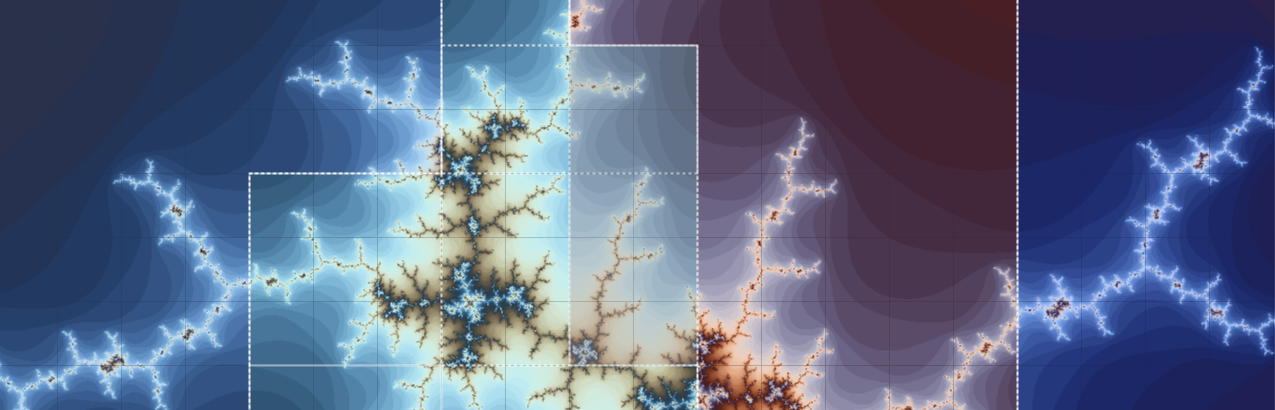
\includegraphics[width=\linewidth]{img/Implementierung/region_group_error}
	\caption{Überlappende Ränder von gruppierten Teilregionen, durch inkorrekte Berechnung des Randes der türkisen Region
	}\label{fig:regionGroupError}
\end{figure}
Bei der Verwendung vieler Worker \( > 10 \) kommt es zu einer unübersichtlichen Darstellung
dieser, da die Aufteilung jedes Workers, sowie dessen Warte- und Rechenzeit separat dargestellt werden.
Deshalb ist eine Gruppierung der einzelnen Worker implementiert, welche alle vom Backend erzeugeten Worker
nach der näher der von ihnen berechneten Regionen auf der Komplexen Ebene hierarchisch zusammenfasst. Dabei kann eine maximale
Anzahl darzustellender Gruppen spezifiziert werden, welche als Grundlage zur Berechnung der Gruppengröße dient (Standardmäßig \( = 4 \)).
Diese erzeugen Gruppen werden dann äquivalent zu einer einzelnen Region im Rest des Frontends behandelt.

Da der \verb|WorkerLayer| für jede Gruppe die von dieser berechnete Fläche auf der komplexen Ebene anzeigt,
muss für eine Gruppe, die aus mehr als einer Region besteht der Rand aller in ihr enthaltenen Flächen berechnet werden.
Dies wurde mit dem \textit{Graham Search}\cite{Cormen} Algorithmus für das Berechnen einer konvexen Hülle implementiert.
Da die gruppierten Regionen jedoch nicht immer konvex sein müssen, muss dieser Algorithmus für ie Berechnung einer konkaven Hülle erweitert
werden, was sich als sehr aufwendig herausgestellt hat und deshalb nur durch eine Vereinfachung implementiert wurde.
Dadurch kann es bei der Darstellung der Gruppierungen im Frontend zu überlappenden Regionsdarstellungen im \verb|WorkerLayer| kommen (siehe \autoref{fig:regionGroupError}).

\subsubsection{Visualisierung}
Die Struktur der Parallelisierung wird in einem Netzwerkgraphen unter dem Fraktal dargestellt.
Mithilfe der Bibliothek \verb|visjs|\footnote{\url{http://visjs.org/}} wird hierzu ein
Graph (siehe \autoref{fig:networkView}) mit 3 Ebenen erzeugt:

Auf der linken Seite befindet sich ein Knoten in Form eines Programmfensters, der das Browserfrontend darstellt.
In der Mitte wird ein Knoten für den Backend-Host mit \enquote{Serverrack} als Symbol dargestellt, der mit dem Frontendknoten verbunden ist.
Auf der rechten Seite befindet sich schließlich zwischen 2 und 4 Knoten, die jeweils eine Gruppe an Arbeitern
darstellen, welche wiederum direkt mit dem Host verbunden sind.

Das Darstellen diesen Graphen wird nach Erhalt jeder Regionsaufteilung des Backends vorgenommen,
sowie die Größe der Leinwand dynamisch an die Anzahl an Knoten angepasst.

\subsubsection{Visualisierung der Rechenzeiten} % components/
Die zeitbezüglichen Komponenten der Visualisierung werden mithilfe der Diagrammfunktionen
der Bibliothek \verb|chartjs|\footnote{\url{http://www.chartjs.org/}} dargestellt
\begin{figure*}[t!]
	\begin{subfigure}[t]{0.3\textwidth}
		\centering
		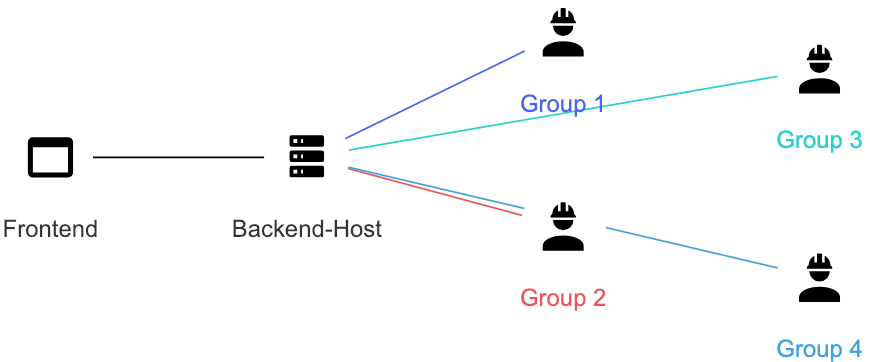
\includegraphics[width=\linewidth]{img/Implementierung/NetworkView}
		\caption{Architektur der Anwendung als Graph
		}\label{fig:networkView}
	\end{subfigure}
	\begin{subfigure}[t]{0.3\textwidth}
		\centering
		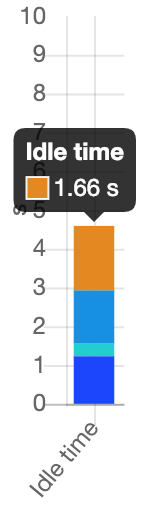
\includegraphics[height=.5\linewidth]{img/Implementierung/IdleTime}
		\caption{Wartezeiten für 5 Gruppen}
		\label{fig:idleTime}
	\end{subfigure}%
	\begin{subfigure}[t]{0.3\textwidth}
		\centering
		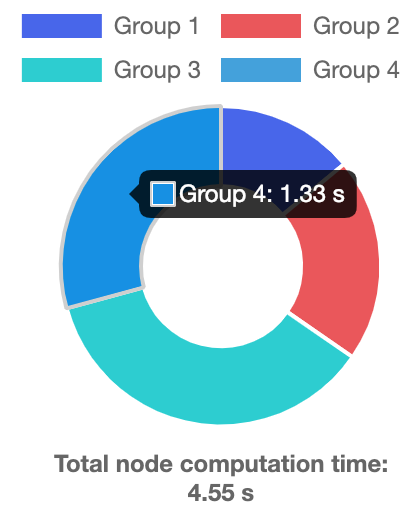
\includegraphics[height=.5\linewidth]{img/Implementierung/ComputationTime}
		\caption{Rechenzeiten für 4 Gruppen}
		\label{fig:computationTime}
	\end{subfigure}
	\caption{Komponenten zur Visualisierung der Rechenzeiten im Frontend}
\end{figure*}


\paragraph{Wartezeit}
Falls einer der Worker vor den anderen mit der Berechnung fertig wird, wartet dieser,
bis er einen neuen Auftrag erhält. Dies ist somit verwschwendete Zeit, welche in einem Balkendiagramm dargestellt wird.
Dabei wird die Differenz zwischen der Rechenzeit aller Knoten und dem am längsten rechnenden Knoten
aufsummiert und nach Gruppe sortiert darstellt (siehe \autoref{fig:idleTime}).

Die Darstellung wird bei Empfang einer Regionsaufteilung (mithilfe \verb|registerRegion| in \verb|WebSocketClient|)
initialisiert indem die Anzahl an Knoten und die Gruppen gespeichert, die Rechenzeit der Knoten auf \( 0 \) gesetzt und
alle Knoten als aktiv markiert werden.
Da die tatsächliche Rechenzeit erst am Ende der Berechnung mit den Regionsdaten selbst verfügbar ist,
wird mithilfe eines Intervalls die Rechenzeit live abgeschätzt, indem sie alle \( 50ms \) um
\( 50ms \) hochgezählt wird, falls die Regionsdaten des Knotens noch nicht empfangen wurden.

\paragraph{ComputationTime}
Zur Darstellung des relativen Verhältnisses der Rechenzeiten wird in einem Kuchendiagramm
die absolute Rechenzeit der Gruppen dargestellt (siehe \autoref{fig:computationTime}).
Dies setzt die benötigte Rechenzeit einer Region in ein Verhältnis zu allen anderen Regionen,
wobei möglichst gleichverteilte Stückgrößen eine gute Aufteilung durch die Lastbalancierung darstellen.

Falls eine Gruppierung der Regionen stattgefunden hat, wird die Summe der Rechenzeiten der einzelnen Regionen 
in einer Gruppe verwendet.
